\documentclass{article}

\usepackage{graphicx}
\usepackage{tikz}
\usepackage{tikzsymbols}
\usetikzlibrary{calc,patterns,shapes.geometric}
\pagestyle{empty}
\usepackage[margin=0pt]{geometry}
\geometry{papersize={14in,12in}}

\def\centerarc[#1](#2)(#3:#4:#5){\draw[#1] ($(#2)+({#5*cos(#3)},{#5*sin(#3)})$) arc (#3:#4:#5);}

\begin{document}
	\begin{figure}
		\centering
		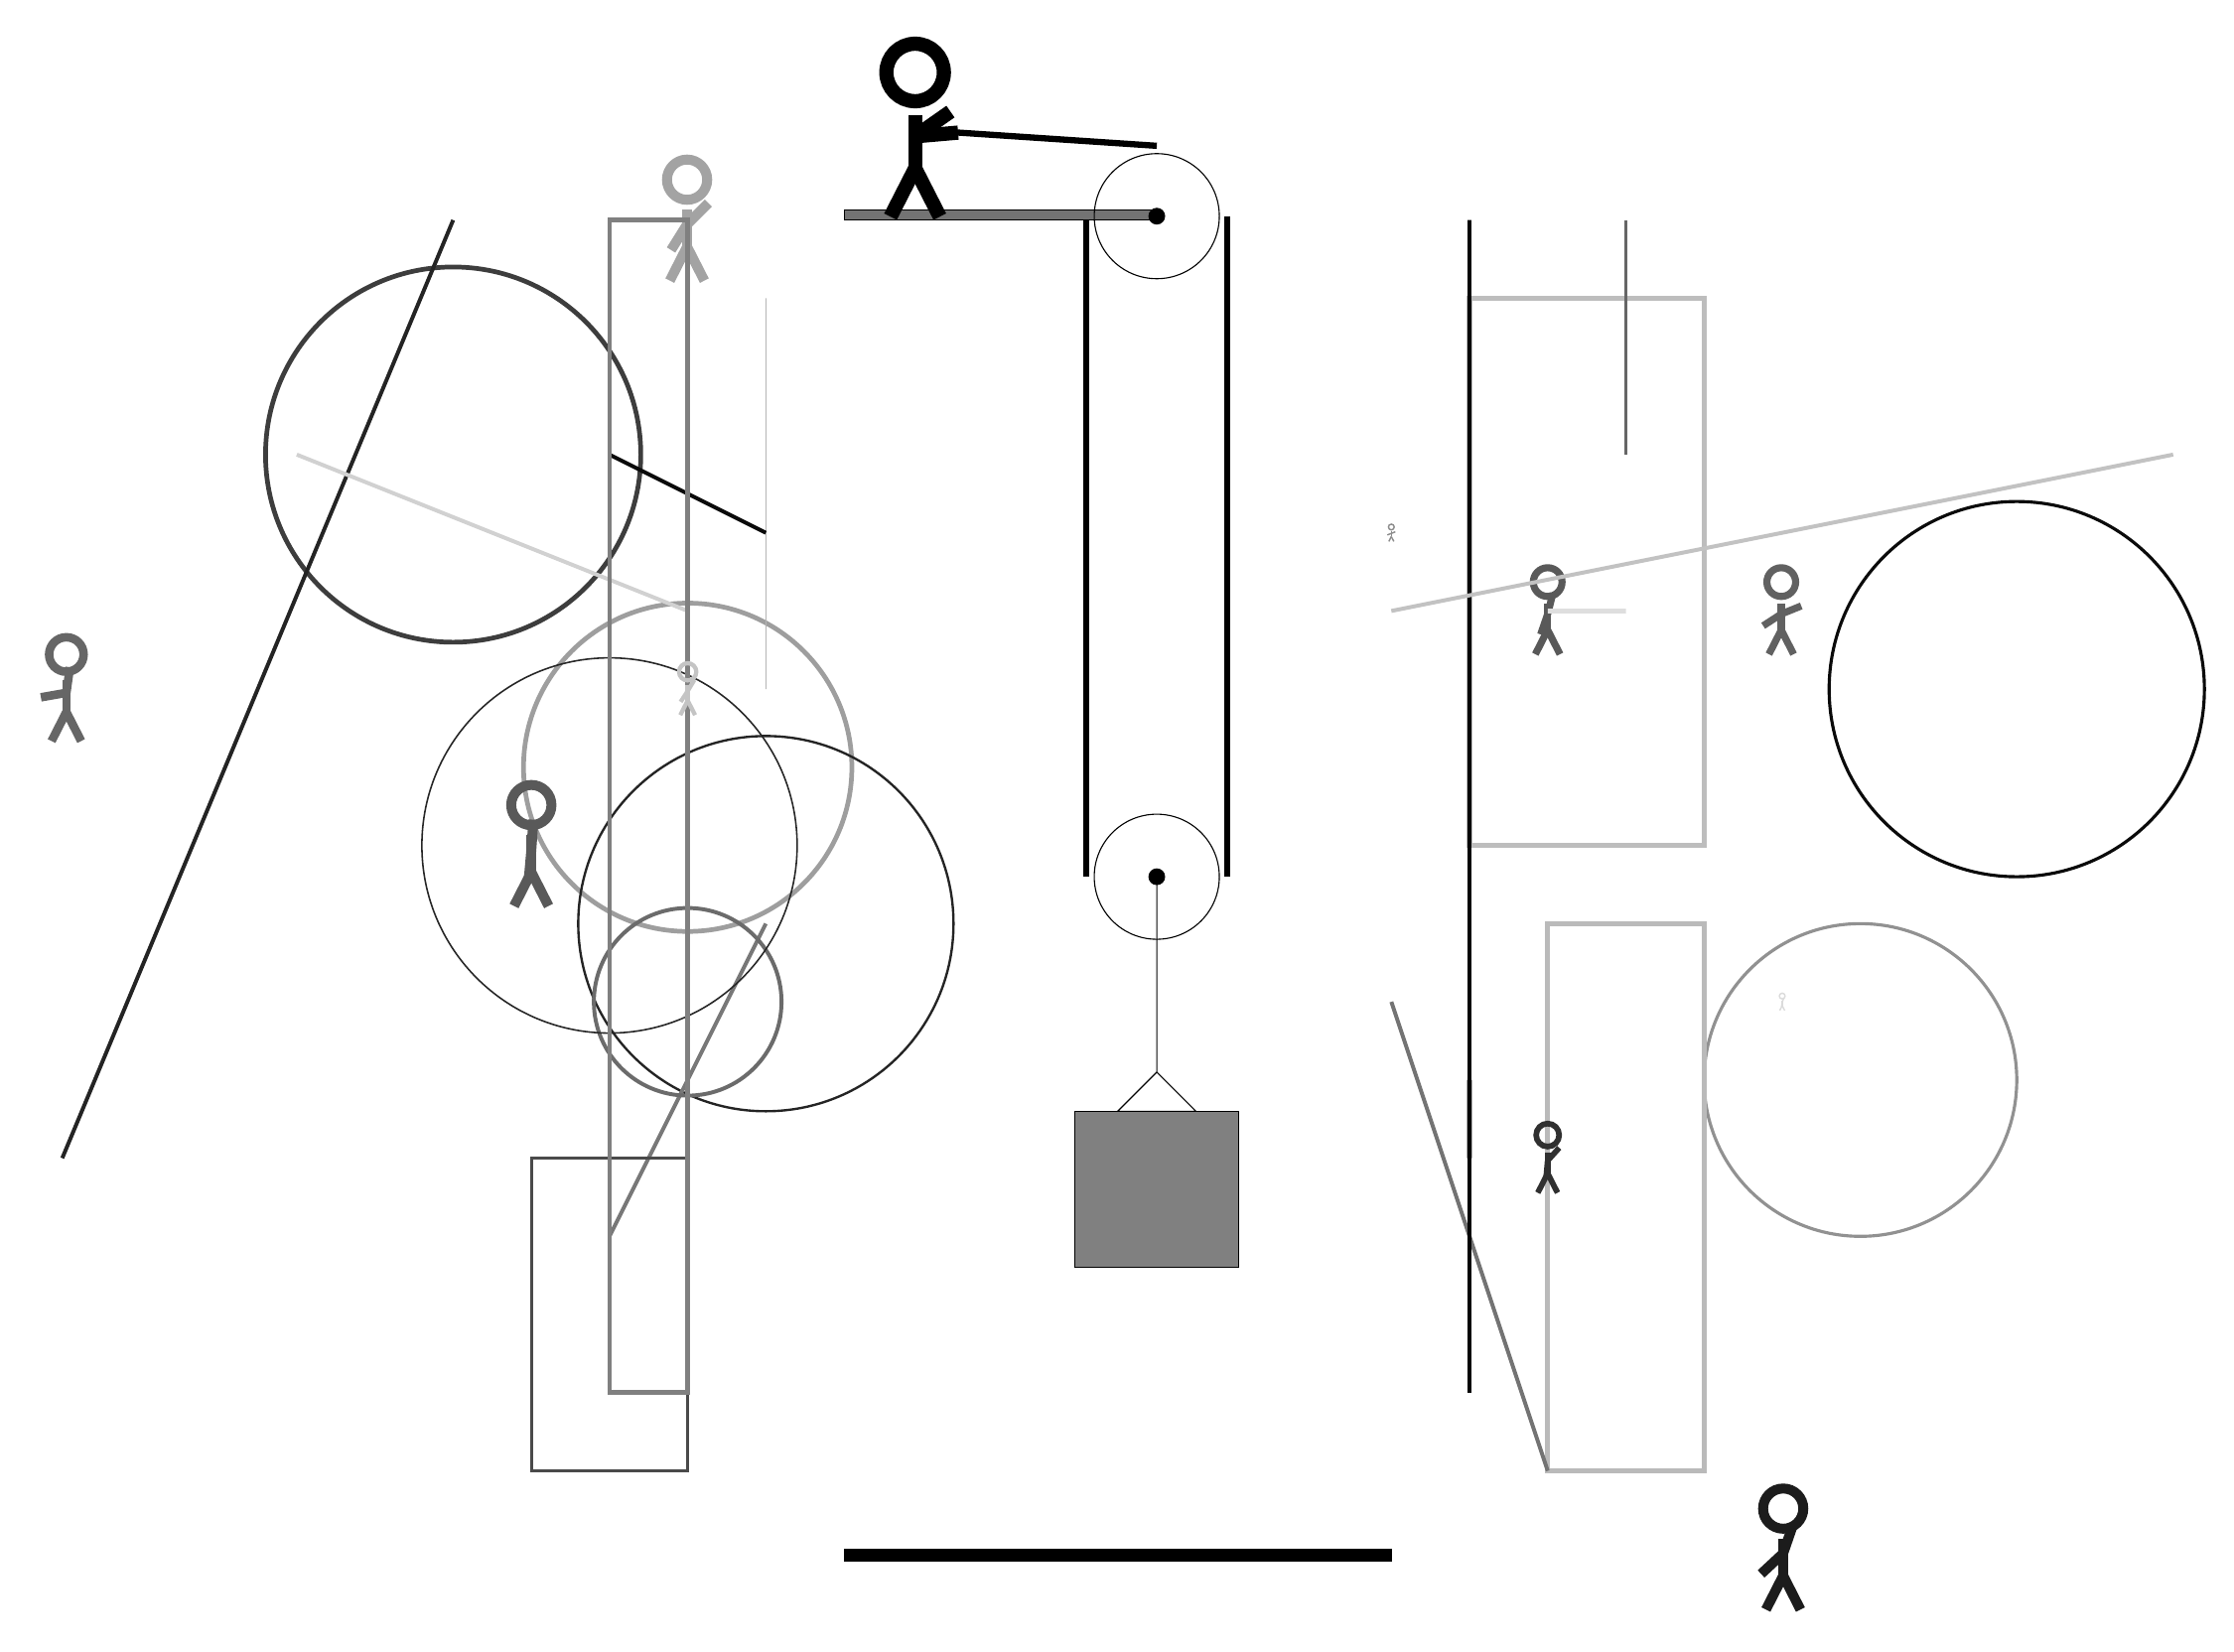
\begin{tikzpicture}
			%%%%% START %%%%%
			
			\draw[fill=black!55] (-2, 14) rectangle (2, 14.125);
			
			\draw (2, 5.6) circle (0.8);
			\draw[fill=black] (2, 5.6) circle (0.1);
			
			\draw (2, 14.05) circle (0.8);
			\draw[fill=black] (2, 14.05) circle (0.1);
			
			\draw (2, 5.6) -- (2, 3.1) -- (1.5, 2.6) -- (2.5, 2.6) -- (2, 3.1);
			\draw[fill=black!50] (0.95, 2.6) rectangle (3.05, 0.6);
			
			\draw [line width=0.6mm, color=black!38](-4, 7) circle (2.1);
			
			\node[line width=0.6mm, color=black!60] at (-12, 8) {\Strichmaxerl[6][10][82]};
			\node[line width=0.3mm, color=black!45] at (5, 10) {\Strichmaxerl[1][21][22]};
			\node[line width=0.2mm, color=black!65] at (7, 9) {\Strichmaxerl[5][71][76]};
			
			\draw [line width=0.3mm, color=black!86](-3, 5) circle (2.4);
			\draw[line width=0.2mm, color=black!29] (-3, 13) rectangle (-3, 8);
			\draw [line width=0.4mm, color=black!43](11, 3) circle (2.0);
			\node[line width=0.6mm, color=black!65] at (-6, 6) {\Strichmaxerl[7][85][86]};
			\draw[line width=0.6mm, color=black!56] (6, 4) rectangle (6, 1);
			\draw[line width=0.6mm, color=black!27] (7, -2) rectangle (9, 5);
			
			\node[line width=0.6mm, color=black!36] at (-4, 14) {\Strichmaxerl[7][58][45]};
			\draw [line width=0.6mm, color=black!76](-7, 11) circle (2.4);
			\draw[line width=0.5mm, color=black!53](-3, 5) -- (-5, 1);
			
			\draw[line width=0.5mm, color=black!86](-7, 14) -- (-12, 2);
			\draw[line width=0.7mm, color=black!26] (6, 13) rectangle (9, 6);
			\draw [line width=0.5mm, color=black!58](-4, 4) circle (1.2);
			\draw [line width=0.2mm, color=black!85](-5, 6) circle (2.4);
			\draw [line width=0.6mm, color=black!61](10, 4) circle (0.0);
			\draw[line width=0.4mm, color=black!71] (-4, -2) rectangle (-6, 2);
			
			\draw[line width=0.5mm, color=black!18](-4, 9) -- (-9, 11);
			\draw[line width=0.5mm, color=black!55](7, -2) -- (5, 4);
			
			\draw[line width=0.7mm, color=black!32] (6, 3) rectangle (6, 2);
			
			\node[line width=0.4mm, color=black!62] at (10, 9) {\Strichmaxerl[5][33][22]};
			\draw[line width=0.7mm, color=black!13] (7, 9) rectangle (8, 9);
			\draw[line width=0.5mm, color=black!96](-3, 10) -- (-5, 11);
			\draw[line width=0.6mm, color=black!50] (-4, 14) rectangle (-5, -1);
			\node[line width=0.2mm, color=black!89] at (10, -3) {\Strichmaxerl[7][43][71]};
			\node[line width=0.5mm, color=black!23] at (-4, 8) {\Strichmaxerl[3][57][59]};
			
			\node[line width=0.3mm, color=black!81] at (7, 2) {\Strichmaxerl[4][85][48]};
			\node[line width=0.5mm, color=black!14] at (10, 4) {\Strichmaxerl[1][81][71]};
			\draw[line width=0.5mm, color=black!60](8, 11) -- (8, 14);
			\draw[line width=0.6mm, color=black!98] (6, 14) rectangle (6, -1);
			\draw [line width=0.4mm, color=black!96](13, 8) circle (2.4);
			\draw[line width=0.5mm, color=black!24](5, 9) -- (15, 11);
			
			\draw[line width=0.8mm] (1.1, 14) -- (1.1, 5.6);
			\centerarc[line width=0.8mm](2, 5.6)(180:360:0.9);
			\draw[line width=0.8mm](2.9, 5.6) -- (2.9, 14.05);
			\centerarc[line width=0.8mm](2, 14.05)(0:90:0.9);
			\draw[line width=0.8mm](2, 14.95) -- (-1, 15.15);
			
			\node at (-1, 15.15) {\Strichmaxerl[10][-175][35]};
			
			\draw[fill=black] (-2, -3) rectangle (5, -3.15);
			
			%%%%% END %%%%%
		\end{tikzpicture}
	\end{figure}	
\end{document}